
\textbf{Úvod}  
Táto príručka popisuje inštaláciu, konfiguráciu a používanie systému na rozpoznávanie emocionálnych výrazov tváre v robotickom pracovisku COCOHRIP. Systém využíva kombináciu hardvérových komponentov a metód hlbokého učenia pre klasifikáciu 7 základných emócií v reálnom čase.

\textbf{Hardvérové komponenty}  
\begin{itemize}
\item Robotické pracovisko COCOHRIP s ramenom UR5e
\item Výpočtová jednotka: 
  \begin{itemize}
  \item GPU NVIDIA RTX 3070 (pre trénovanie modelov)
  \item CPU Intel i7 (pre inferenciu v reálnom čase)
  \end{itemize}
\item Senzory:
  \begin{itemize}
  \item Kamera XIMEA xiMU
  \item USB kamera (záložný zdroj)
  \end{itemize}
\end{itemize}

% \begin{figure}[H]
% \centering
% \includegraphics[width=0.8\textwidth]{system_architektura}
% \caption{Bloková schéma hardvérovej architektúry}
% \end{figure}

\textbf{Softvérové prostredie}  
\begin{itemize}
\item Trénovacie prostredie: Ubuntu 24.04 LTS, TensorFlow 2.10, PyTorch 1.12, Docker
\item Produkčné prostredie: Ubuntu 22.04 LTS, \gls{ros}2 Humble, TensorFlow Lite
\end{itemize}

\textbf{Inštalácia systému}  
\begin{enumerate}
\item Naklonovanie repozitára:
\begin{lstlisting}[language=bash]
git clone https://github.com/KocurMaros/master_thesis_practical
cd master_thesis_practical
\end{lstlisting}

\item Zostavenie Docker kontajnera:
\begin{lstlisting}[language=bash]
docker compose build
\end{lstlisting}

\item Spustenie vývojového prostredia:
\begin{lstlisting}[language=bash]
docker compose up
\end{lstlisting}
\end{enumerate}

\textbf{Konfigurácia systému}  
Upravte parametre v súbore \texttt{trainRAF-DB.ipynb}:
\begin{lstlisting}[language=Python]
# Hyperparametre
EPOCHS = 50
BATCH_SIZE = 32
LEARNING_RATE = 1e-4
\end{lstlisting}

\textbf{Spustenie systému}  

Pred spustením systému, je potrebné skontrolovať, či ovladače kamery sú správne nainštalované. V prípade, použitia kamry s Python API, ktoré niesu súčasťou python package managera, je potrebné vytvoriť symlink na ovládače kamery alebo nakopírovať API do virtuálného prostredia.
\begin{lstlisting}[language=bash]
python3 -m venv venv
source venv/bin/activate
pip install -r requirements.txt
cd /path/to/master_thesis_practical/ros_package/facial_expression
sudo chmod +x ./video_stream.sh
sudo chmod +x ./run_facial_expression.sh
./video_stream.sh & ./run_facial_expression.sh
\end{lstlisting}

\textbf{Používanie systému}  
\begin{itemize}
\item Odoberanie emočných predikcií:
\begin{lstlisting}[language=bash]
ros2 topic echo /emotion_prediction
\end{lstlisting}

\item Zobrazenie video streamu:
\begin{itemize}
\item Otvorte prehliadač na \texttt{localhost:5000}
\item Formát streamu: MJPEG 1280x720 @ 30 FPS
\end{itemize}
\end{itemize}

\textbf{Riešenie problémov}  

\begin{tabular}{|p{6cm}|p{9cm}|}
\hline
Problém & Riešenie \\
\hline
Chyba pri inicializácii kamery XIMEA & Skontrolujte oprávnenia používateľa v skupine \texttt{video} \\
Nízka frekvencia predikcií & Znížte rozlíšenie kamery v konfiguračnom súbore \\
\hline
\end{tabular}

\begin{figure}[!htpb]
\centering
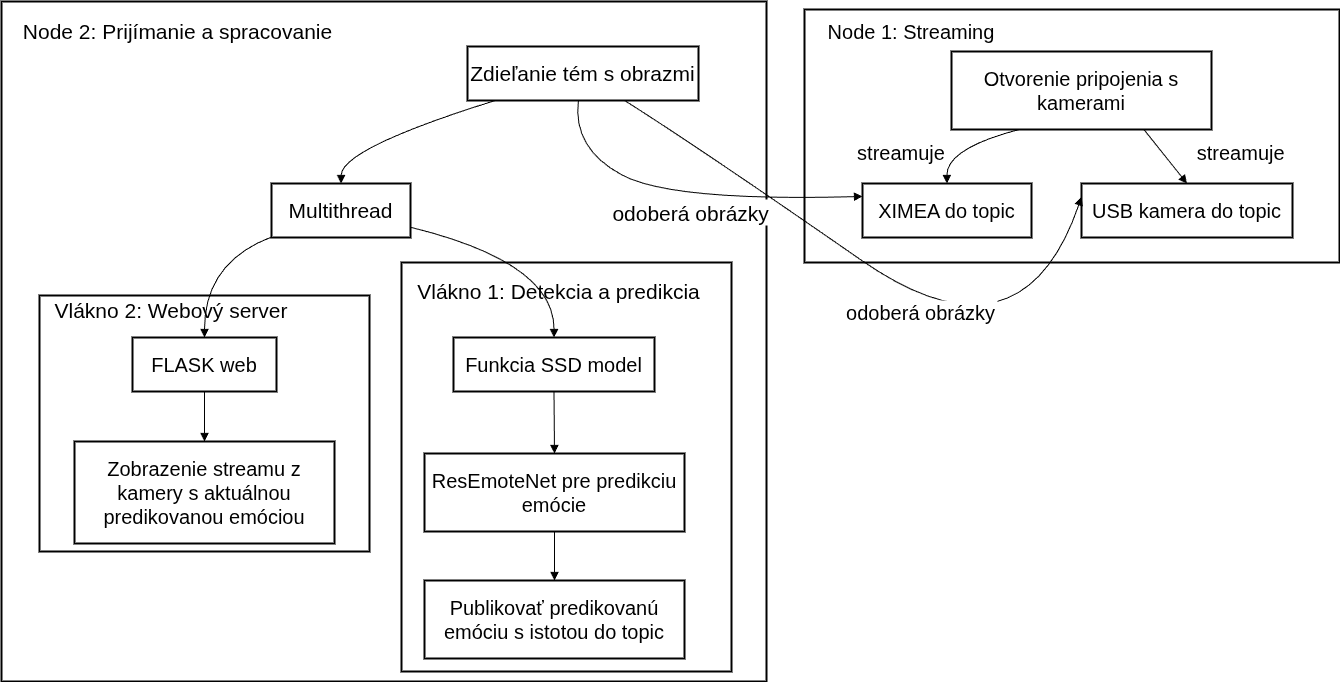
\includegraphics[width=0.8\textwidth]{img/ros2_nodes.png}
\caption{Bloková schéma softvérovej architektúry}
\label{fig:ros2_nodes}
\end{figure}

\begin{itemize}
\item Ukážka výstupu predikcií:
\begin{lstlisting}[language=Python]
EmotionPredictor:
  - timestamp: 1718195100.123456
  - emotion: happy
  - confidence: 92%
\end{lstlisting}
\end{itemize}

